\documentclass[conference]{IEEEtran}
\usepackage{cite}
\usepackage{amsmath,amssymb,amsfonts}
\usepackage{algorithmic}
\usepackage{graphicx}
\usepackage{textcomp}
\usepackage{xcolor}
\usepackage{float}
\usepackage{caption}
\usepackage[numbib]{tocbibind}
\usepackage{pbox}

\graphicspath{{./img2/}{./images/25_50/}{./images/1_25/}}
\begin{document}
\title{COMP90086 Computer Vision Final Project\\
Stereo Disparity
}
\author{
\IEEEauthorblockN{Jun Li Chen}
\IEEEauthorblockA{1043258}
\and
\IEEEauthorblockN{Tianli Cheng}
\IEEEauthorblockA{1128434}
}
\maketitle

\thispagestyle{plain}
\pagestyle{plain}

\section{Introduction}
Stereo matching is a process of finding corresponding pixels representing the same point in 3--D reality from images taken from different angles and positions. The disparity can be calculated by difference between the $x$ pixel coordinate of the right image from the $x$ pixel coordinate of the left image, given that they lie parallel in the image. This is negatively correlated to the depth of the object from the image plane.

Different comparison functions exist for similarity calculation. Our report selects several window--based matching functions and compares their performance over a set of moving vehicle image pairs. Pixels pairs with the highest similarity will be tagged as correspondencing pixel pairs, and the results will be evaluated by computing the root mean square (RMS) and pixel error fractions between the calculated disparity and the ground truth.

\section{Methodology}
\subsection{Implementation}
Before running each image pair through our program to create a disparity map, a bilateral filter smoothing function is applied to the image pairs. This was done to reduce the effect of noise on our disparity map output. Bilateral filter was chosen as it preserves edges in the image while smoothening the image.

The program iterates through pixels on the left image, while creating a sliding window of search size 25 in the right image with pixel index from the left image. The sum of absolute difference (SAD) and the sum of square difference (SSD) are selected as the classic similarity measurement functions to start with.

SAD of block $W1$ and block $W2$ was calculated by sum of intensity differences between corresponding pixel pairs, as in:

\begin{equation*}
    SAD=\sum^{n}_{i=0}\sum^{m}_{j=0}|W1[i,j]-W2[i,j]|
\end{equation*}

Similarly, the SSD of block $W1$ and block $W2$ was calculated by summing up the square of intensity differences between each corresponding pixel pairs, as in:

\begin{equation*}
    SSD=\sum^{n}_{i=0}\sum^{m}_{j=0}(W1[i,j]-W2[i,j])^2
\end{equation*}

Between SSD and SAD, SSD is more discriminative compared to SAD since the differences between image patches are amplified through squaring [1]. In case there given a pixel with a value difference much larger compared to the rest in the block, SSD will score it higher than SAD does. This means that the pixels with small differences are more likely to be ignored by SSD.

The pixel index with the lowest difference value in the sliding window to the original pixel on the left image is used as the pixel index to calculate the value of pixel shift as the disparity value for said pixel.
\
\subsection{Evaluation}

In the output disparity map with a pixel block size of 1 and search size of 25 as shown in Figure 1 below, there are many small adjacent areas of high and low disparity, resulting in a detailed disparity output, albeit with a significant amount of noise, especially near the bottom of image, which represents the road in the original input image pairs. 

\begin{figure}[H]
    \centering
    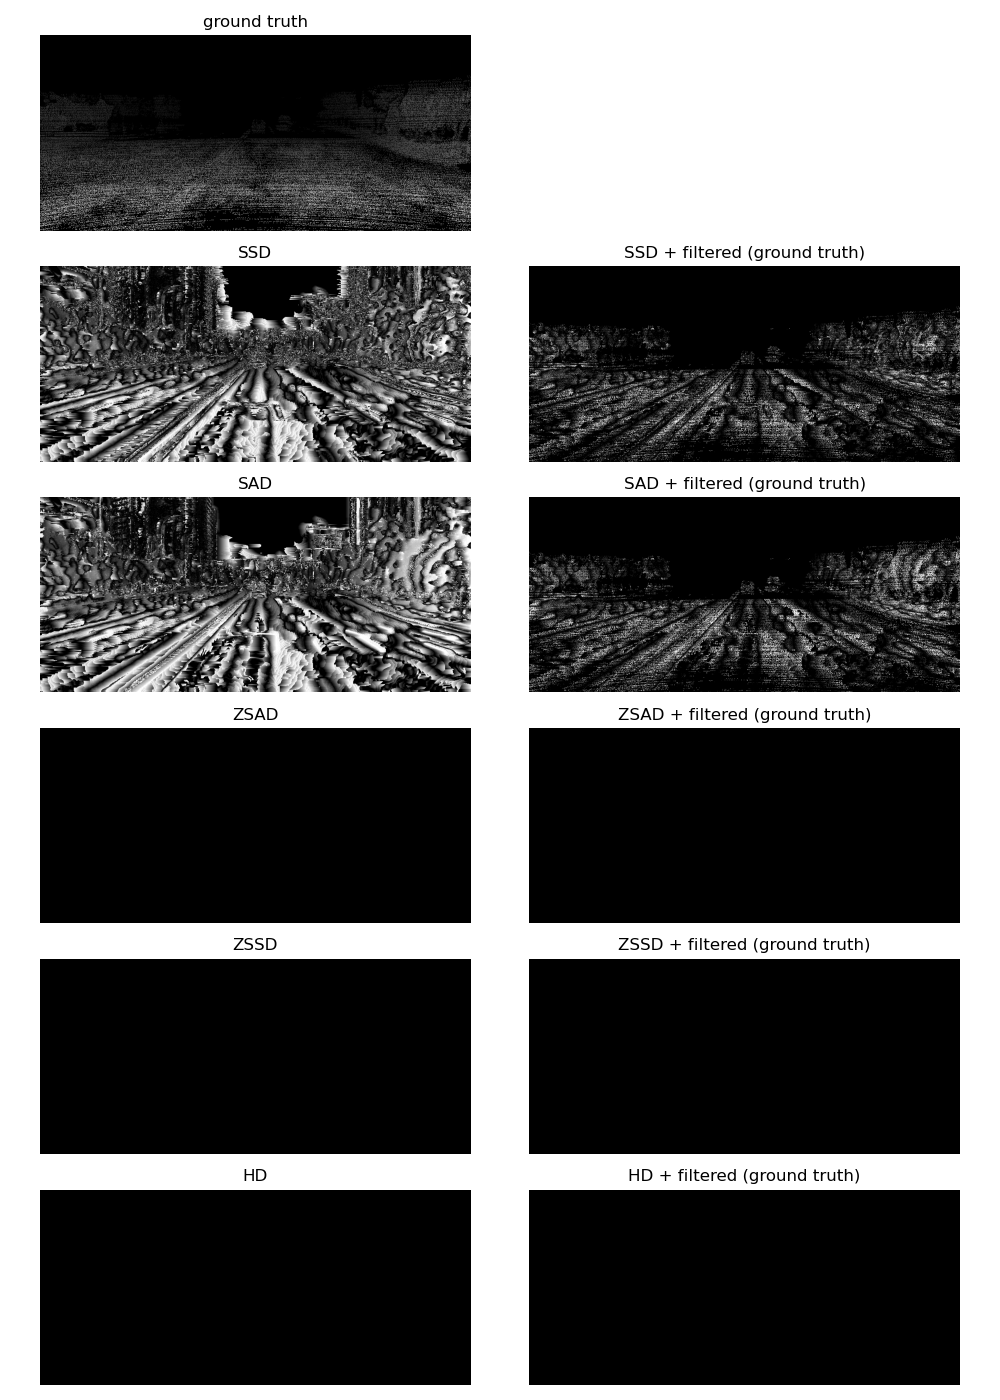
\includegraphics[width=8.8cm]{702_output_1_25.png}
    \captionof{figure}{Disparity map output with pixel block size of 1 \& sliding window search size of 25.}
\end{figure}

This results in high RMS value and low pixel error fractions as in Figure 2 below. This can be caused by residual noise in the image, or the small size of the sliding search window. The time taken for SSD and SAD function to complete the disparity map calculation is also very high at around 90\(\sim \)95 seconds for each image.

\begin{figure}[H]
    \centering
    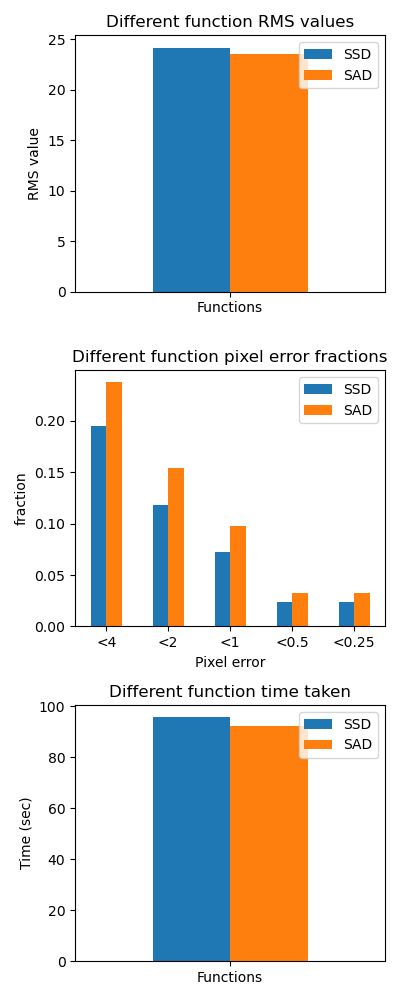
\includegraphics[height=12cm]{702_stats_1_25.png}
    \captionof{figure}{Disparity performance with pixel block size of 1 \& sliding window search size of 25.}
\end{figure}

\section{Improvement}

\subsection{Implementation}

Due to the low performance and slow program runtime, the original program was modified to interface with different comparison functions including zero mean sum of absolute difference (ZSAD), zero mean sum of squared difference (ZSSD) and Hamming distance of census transform (HD). Furthermore, instead of iterating through each individual pixel to calculate each disparity value, the modified program iterates through blocks of size $n$ by $n$ pixels, comparing it with the corresponding sliding window search block with the same height $n$. 

For example, we used a pixel block size of 25 (width 25, height 25) on the left image, while searching through the right image with a sliding window of size 50 (width 50, height 25). We assume there is no vertical disparity between the image pairs, therefore only the width of the sliding window is varied.

ZSAD and ZSSD were chosen due to these comparison functions' ability to perform some degree of normalization to avoid bios towards large values in the resulting output. The ZSAD between pixel blocks of image pairs is calculated by the sum of the deviation differences between each corresponding pixel pairs, as in:

\begin{equation*}
    \begin{aligned}
        ZSAD= {} & \sum^{n}_{i=0}\sum^{m}_{j=0}|(W1_{[i,j]}-\frac{1}{nm}\sum^{n}_{i=0}\sum^{m}_{j=0}W1_{[i,j]})\\
        & -(W2_{[i,j]}-\frac{1}{nm}\sum^{n}_{i=0}\sum^{m}_{j=0}W2_{[i,j]})|
    \end{aligned}
\end{equation*}

In ZSAD, the differences between each element and the mean intensity value in both image blocks is first calculated, before finding the absolute difference of the corresponding deviations. Similarly, ZSSD was calculated by summing up the square of deviation differences between each corresponding pixel pairs, as in:

\begin{equation*}
    \begin{aligned}
        ZSSD= {} & \sum^{n}_{i=0}\sum^{m}_{j=0}((W1_{[i,j]}-\frac{1}{nm}\sum^{n}_{i=0}\sum^{m}_{j=0}W1_{[i,j]})- \\
        & (W2_{[i,j]}-\frac{1}{nm}\sum^{n}_{i=0}\sum^{m}_{j=0}W2_{[i,j]}))^2
    \end{aligned}
\end{equation*}

By only preserving the deviation, these comparison functions are less sensitive to a general shift in intensity which can be caused by a change in lightning. However, normalization can be taken further by including the relation of a single pixel with the image block it belongs to into consideration. Normalized Cross--Correlation (NCC) is one of the most classic metrics including local relations when mapping similarity between images. It is less sensitive to a linear change in lightning intensity but computationally expensive [3]. Hence, HDCT has been chosen as an alternative to NCC, which also normalizes image patterns through local correlation. 

The census transform records each pixel with a lower intensity compared to the center pixel as 0 and the rest as 1. Figure 3 below gives an example of how this census transform works in a 3 by 3 window.

\begin{figure}[H]
    \centering
    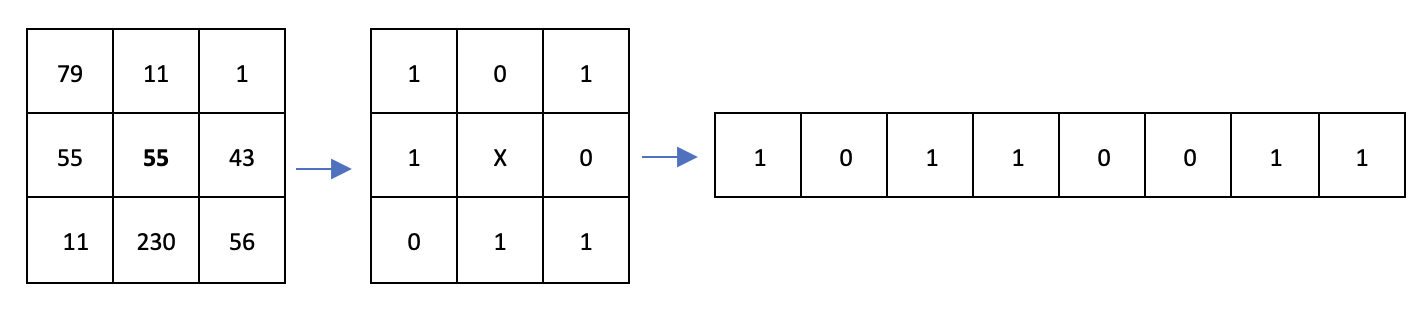
\includegraphics[width=8cm]{fig1.png}
    \caption{Census transform}
\end{figure}

This represents each pixel's relation to the center pixel in a binary form. Therefore, it is non--parametric and insensitive to radiometric variations [2].

The Hamming distance of the census transform between two blocks is calculated by performing an XOR operation on the two 1--D binary representations. By counting the number of 1s existing in the outcome of XOR between blocks, the resulting output represents the number of different patterns. Figure 4 below shows a simple example of how it works.

\begin{figure}[H]
    \centering
    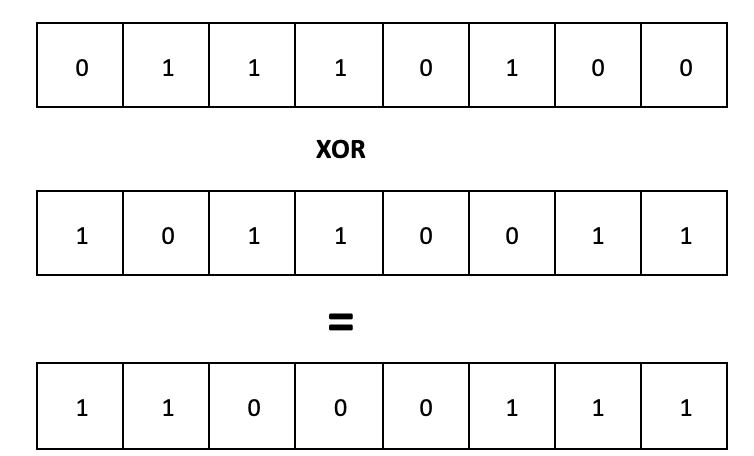
\includegraphics[width=6cm]{fig2.png}
    \caption{Hamming distance of Census transform}
\end{figure}

\subsection{Evaluation}

In the output disparity map with a pixel block size of 25 and search size of 50 as shown in Figure 5 below, while the output disparity map looks more 'pixelated', the disparity representation is much closer to our ground truth, with pixel which are 'closer' represented by higher colors, and vice versa, pixels which are more 'distant' represented by darker colors.

\begin{figure}[H]
    \centering
    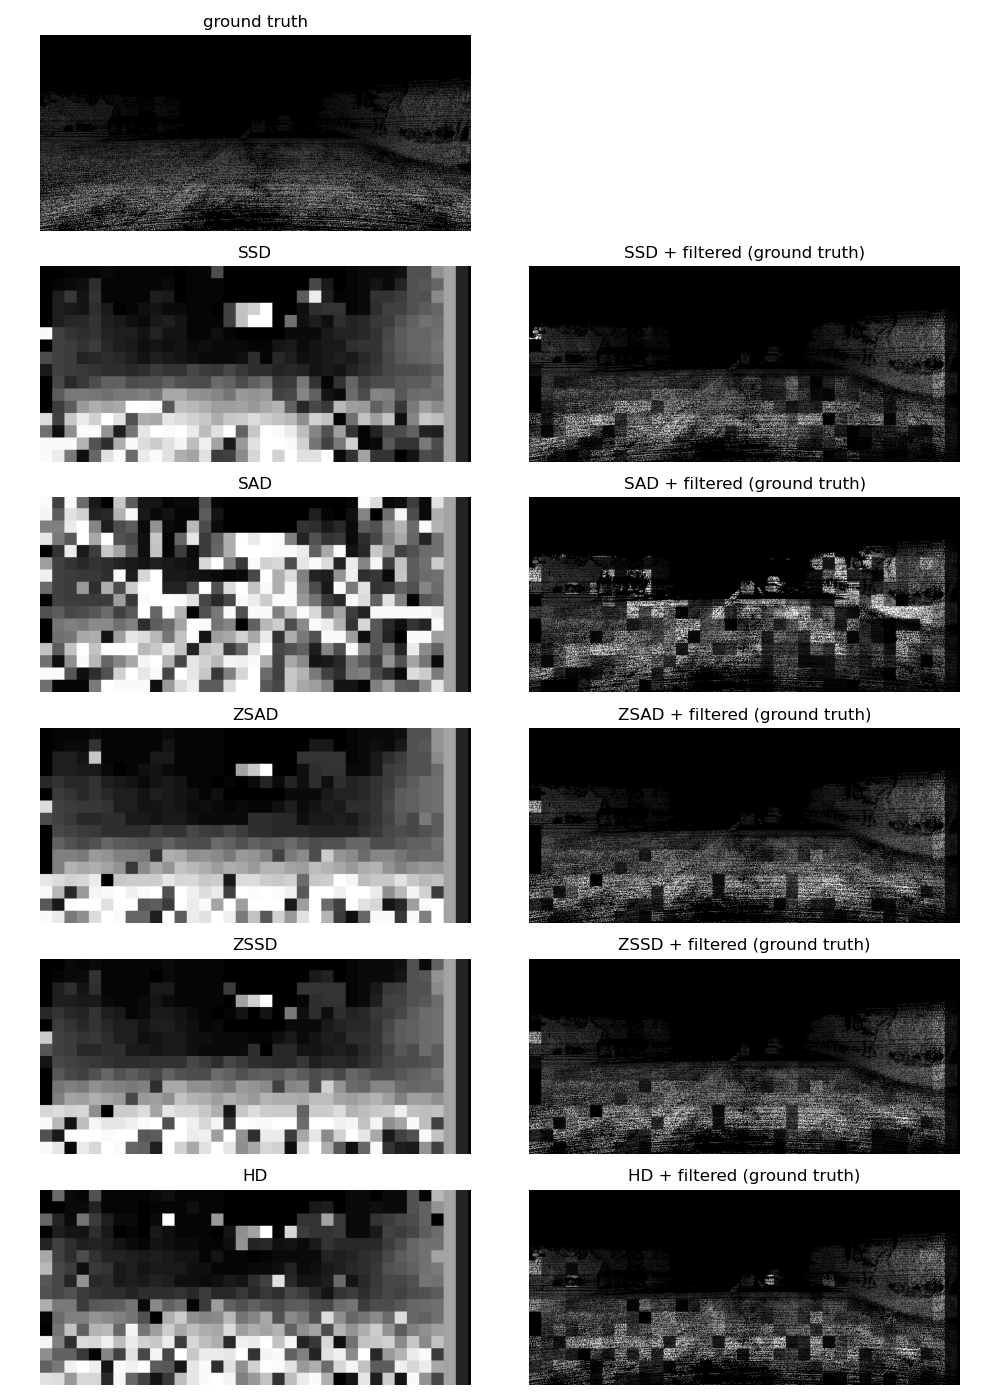
\includegraphics[width=8.8cm]{702_output_25_50.png}
    \captionof{figure}{Disparity map output with pixel block size of 25 \& sliding window search size of 50.}
\end{figure}

After running our improved program through the entire suit of image pairs, the result was a much lower mean RMS value and much higher mean pixel error fractions as in Figure 2 below. 
The time taken for the different comparison functions to complete the
disparity map calculation is significantly reduced to between 0.4\(\sim\)1.6 seconds per image pair.

\begin{figure}[H]
    \centering
    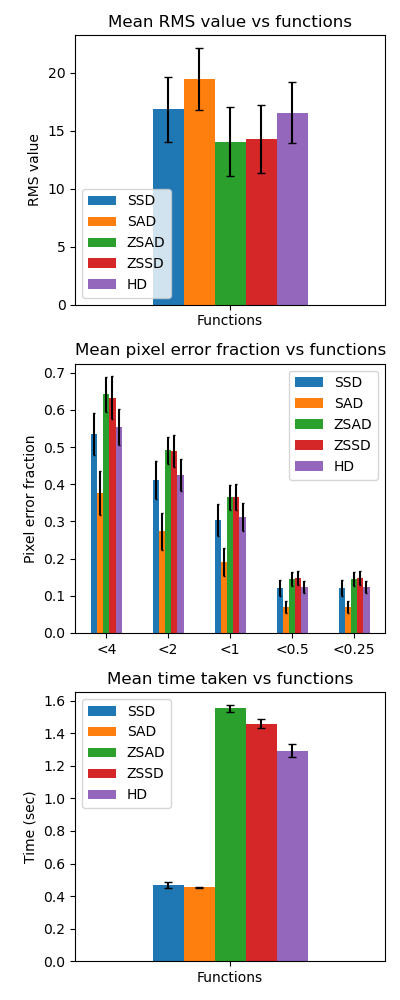
\includegraphics[height=12cm]{stats_25_50.png}
    \captionof{figure}{Disparity performance with pixel block size of 25 \& sliding window search size of 50. (See Table I, II and III for bar chart values)}
\end{figure}

\begin{center}
    \begin{tabular}{l c c c c c}
        \textbf{Function} & \textbf{SSD} & \textbf{SAD} & \textbf{ZSAD} & \textbf{ZSSD} & \textbf{HD} \\ [0.5ex] 
        Mean & 16.85 & 19.45 & 14.06 & 14.29 & 16.53 \\
        SD & 2.79 & 2.66 & 2.99 & 2.91 & 2.62
    \end{tabular}
    \captionof{table}{RMS statistic table values.}
\end{center}
\begin{center}
    \begin{tabular}{l c c c c c}
        \textbf{Function} & \textbf{SSD} & \textbf{SAD} & \textbf{ZSAD} & \textbf{ZSSD} & \textbf{HD} \\ [0.5ex] 
        Mean ($<4$) & 0.536 & 0.376 & 0.642 & 0.634 & 0.555 \\
        Mean ($<2$) & 0.411 & 0.273 & 0.491 & 0.490 & 0.425 \\
        Mean ($<1$) & 0.303 & 0.192 & 0.365 & 0.366 & 0.313 \\
        Mean ($<0.5$) & 0.120 & 0.071 & 0.145 & 0.148 & 0.123 \\
        Mean ($<0.25$) & 0.120 & 0.071 & 0.145 & 0.148 & 0.123 \\
        & & & & & \\
        SD ($<4$) & 0.057 & 0.057 & 0.046 & 0.057 & 0.049 \\
        SD ($<2$) & 0.050 & 0.050 & 0.036 & 0.042 & 0.042 \\
        SD ($<1$) & 0.043 & 0.038 & 0.033 &  0.035 & 0.037 \\
        SD ($<0.5$) & 0.022 & 0.016 & 0.018 & 0.019 & 0.016 \\
        SD ($<0.25$) & 0.022 & 0.016 & 0.018 & 0.019 & 0.016 \\
    \end{tabular}
    \captionof{table}{Pixel error fraction statistic table values.}
\end{center}
\begin{center}
    \begin{tabular}{l c c c c c}
        \textbf{Function} & \textbf{SSD} & \textbf{SAD} & \textbf{ZSAD} & \textbf{ZSSD} & \textbf{HD} \\ [0.5ex] 
        Mean & 0.466 & 0.453 & 1.553 & 1.460 & 1.294 \\
        SD & 0.019 & 0.004 & 0.022 & 0.028 & 0.042
    \end{tabular}
    \captionof{table}{Time taken statistic table values.}
\end{center}

\section{Analysis}

It was found that the computation time of pixel--wise disparity calculation is extremely long in this case since image pairs from our dataset are of size 400 pixels by 881 pixels. The function will iterate $400*881*881=310464400$ times if it searches every pixel on the left image and finds correspondence on the right image on the same line. The iteration must be deducted to improve the program's performance to be feasible for real--time applications.

By setting a search size, the program will not iterate over all pixels laying on the same line on the right image but only within a defined searching window of fixed size (example: search size of 25 pixels). Meanwhile, the function will search those image blocks with center coordinates closer to the original coordinate of the block cropped from the left image first, since the correspondence is more likely to be found in those locations. This brings the total iterations performed down to $400*881*25=8810000$, improving the performance of our original implementation by a factor of 35.

The number of iterations can be further reduced by assuming each pixel in the image block holds the same disparity. By replacing pixel--wise correspondence searching with block--wise correspondence searching, the maximum number of iterations becomes:

\begin{equation*}
    \frac{400*881*(window\_size-block\_width)}{block\_width*block\_height}
\end{equation*}

With a pixel block size of 25, and search window size of 50, the resulting number of iterations needed to be performed reduces to just $\frac{400*881*(50-25)}{25*25}=14096$ iterations, representing a performance increase by a factor of 22025 over our original naive pixel iteration implementation.

\vspace{4pt}
\section{Conclusion}

SSD and SAD functions perform the fastest, due to the lower number of total calculations needed to be performed. While the ZSAD and ZSSD functions have much longer runtime due to more calculations performed (3--4 times as much time as SSD and SAD), the output has a lower RMS value and percentage of pixel error fraction, proving to be good choices for estimating more accurate disparity maps, while SSD is better at generating an acceptable disparity map with much less overhead. 

HDCT has a slightly lower computational cost compared to ZSAD and ZSSD since the operation is more simple and can be performed bitwise. However, this report uses the NumPy operation instead of the bit operation to avoid increasing the number of total iterations to perform a bitwise comparison. The RMS of HDCT is not as high as ZSAD and ZSSD. The reason behind it might be that certain information is lost while conducting the census transformation on image blocks. The local relations have been classified binarily according to the comparison between each element and the central element while ZSAD and ZSSD maintain more information on correspondences. It loses global information as the cost of considering local patterns while maintain low computational complexity.  

We observed that with increasing the pixel block size, comparison function runtime decreases significantly, while the disparity map output performs worse after a certain pixel block size. Pixel block size of 25 proves to be a good middle ground, as the disparity map output has the lowest RMS value, with the comparison functions running between 0.5--2sec to complete.

\begin{center}
    \begin{tabular}{l c c c}
        \pbox{4cm}{\textbf{Comparison} \\ \textbf{function}} & \textbf{Runtime} & \textbf{RMS} & \pbox{4cm}{\textbf{Pixel error} \\ \textbf{fractions ($<1$)}} \\ [2ex]
        SSD & 0.4 sec & 17.6 & 0.31 \\
        SAD & 0.4 sec & 19.5 & 0.19 \\
        ZSAD & 1.6 sec & 14.3 & 0.36 \\
        ZSSD & 1.5 sec & 14.5 & 0.35 \\
        HD & 1.3 sec & 17.4 & 0.32 
    \end{tabular}
    \captionof{table}{Different comparison function performance based on pixel block size of 25, sliding window search size of 50.}
\end{center}

\begin{center}
    \begin{tabular}{c c c c}
        \pbox{4cm}{\textbf{Pixel block} \\ \textbf{size}} & \pbox{4cm}{\textbf{Sliding window} \\ \textbf{search size}} & \textbf{Runtime} & \textbf{RMS} \\ [2ex]
        1 & 25 & 187.0 sec & 22.1 \\
        9 & 49 & 2.9 sec & 18.4 \\
        25 & 50 & 0.5 sec & 16.6 \\
        49 & 98 & 0.4 sec & 19.7
    \end{tabular}
    \captionof{table}{Different pixel block size and sliding window search size performance based on SSD comparison function.}
\end{center}

In the end, we chose a pixel block size of 25 and the zero mean sum absolute difference as our final program implementation as it achieves of good balance between output performance and efficient runtime, a significant improvement over our original implementation.

\section{Final Thought}

Since our implementation was done in a Jupyter notebook in Python, the program was majorly bottlenecked due to running only in a single process. Most of the block comparison calculations could in theory be parallelized for better performance with opportunities for real time applications such as advanced driver assistance systems (ADAS) in automotives. The idea to parallelize calculations using multiple processes was theorized early, but not implemented due to time \& difficulty constraints of the project.

\newpage
\begin{thebibliography}{00}
\bibitem{1} Schmidt, A., Kraft, M. and Kasiński, A., 2010. An Evaluation of Image Feature Detectors and Descriptors for Robot Navigation. Computer Vision and Graphics, pp.251-259.
\bibitem{2} Sarika, S., Deepambika, V. and Rahman, M., 2015. Census Filtering Based Stereomatching under Varying Radiometric Conditions. Procedia Computer Science, 58, pp.315-320.
\bibitem{3} Tsai, D. and Lin, C., 2003. Fast normalized cross correlation for defect detection. Pattern Recognition Letters, 24(15), pp.2625-2631.
\end{thebibliography}

\end{document}
